
\begin{frame}
    \frametitle{Locomoción}
    \small

    \begin{block}{Locomoción}
        Traslación de un lugar a otro.
    \end{block}

    El humano copia a la naturaleza para construir tipos de locomoción.
    \TODO{Mostrar ejemplos del libro Figura 2.1. animales y robots reales.}

    \begin{center}
        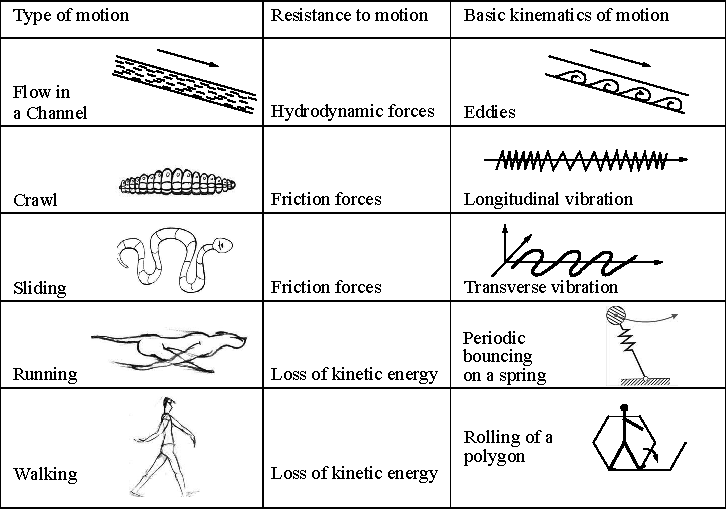
\includegraphics[width=0.7\columnwidth]{images/biological_locomotion_systems.pdf}
    \end{center}

    La naturaleza tuvo que adaptar a los animales para terrenos irregulares!

    \note{Los insectos por ejemplo tienen que sortear cambios de altura que superan en ordenes de magnitud su tamaño.}

    Utilizamos ruedas por que son muy eficientes en terrenos planos y firmes.
\end{frame}


\begin{frame}
    \frametitle{Cinemática y Dinámica}
    \begin{block}{Cinemática}
        La cinemática es la rama de la mecánica que describe el movimiento de los objetos sólidos sin considerar las causas que lo originan (las fuerzas) y se limita, principalmente, al estudio de la trayectoria en función del tiempo. Para ello utiliza velocidades y aceleraciones, que describen cómo cambia la posición en función del tiempo.
    \end{block}
    \note{La velocidad se determina como el cociente entre el desplazamiento y el tiempo utilizado, mientras que la aceleración es el cociente entre el cambio de velocidad y el tiempo utilizado.}

    \begin{block}{Dinámica}
        La dinámica es la parte de la física que estudia la relación existente entre las fuerzas que actúan sobre un cuerpo y los efectos que se producirán sobre el movimiento de ese cuerpo.
    \end{block}

    \note{Los antiguos pensadores griegos creían que la velocidad y la constancia del movimiento en la línea recta de un cuerpo (fenómeno descripto años más tarde como movimiento rectilíneo uniforme o MRU) estaban proporcionalmente relacionadas con una fuerza constante. Por extensión, se creía que la caída de un cuerpo pertenecía a esa categoría, por lo que se suponía que caería más rápido el cuerpo que más pesara.
    \\
    Luego, Galileo Galilei entendió que la caída de los cuerpos no podía ser un movimiento uniforme, y que desde una misma altura, dos cuerpos de distinto peso tardan lo mismo en caer. Este contexto fue lo que posibilitó que algunos años después, Isaac Newton estableciera las tres leyes fundamentales de la dinámica, que explicaban las pautas fundamentales del comportamiento de los cuerpos.}

\end{frame}


\begin{frame}
    \frametitle{Locomoción}

    Manipulación: un brazo robótica está fijo y mueve objetos en su espacio de trabajo aplicando fuerza sobre ellos.

    Locomoción: el entorno está fijo y el robot se mueve impartiendo fuerza sobre el entorno.
    \begin{itemize}
        \item Estabilidad
        \begin{itemize}
            \item Geometría y Número de puntos de contacto
            \item Centro de gravedad
            \item Estabilidad estática y dinámica
            \item Inclinación del terreno
        \end{itemize}
        \item Característica de contacto
        \begin{itemize}
            \item Punto de contacto/ distancia y forma de camino
            \item Ángulo de contacto
            \item Fricción
        \end{itemize}
        \item Tipo de entorno
        \begin{itemize}
            \item Estructura
            \item Medio (agua, aire, terreno suave o firme)
        \end{itemize}
    \end{itemize}
\end{frame}

\begin{frame}
    \frametitle{Locomoción: Robots con patas}

    \begin{center}
        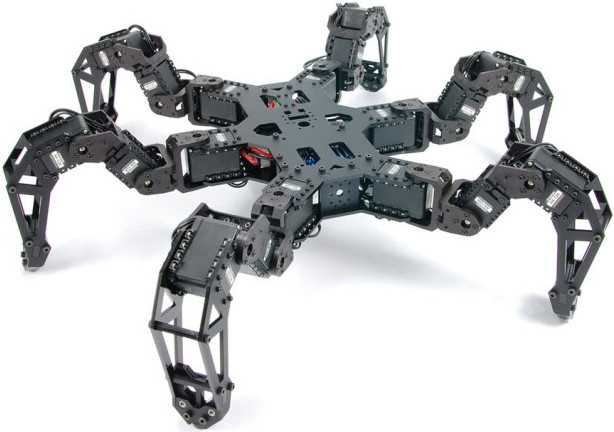
\includegraphics[width=0.4\columnwidth]{images/hexapod_phantomX_mark_II.jpg}
    \end{center}
    \footnotesize
    {\bf Ventajas}:
    \begin{itemize}
        \item Permiten ir por terrenos irregulares
        \item Reducen el impacto ambiental dado que tienen menos puntos de contacto
    \end{itemize}
    {\bf Desventaja: }
    \begin{itemize}
        \item Complegidad mecánica
        \item mayor consumo (una pata con muchos joints puede tener que soportar todo el peso del robot)
        \item para que tenga mucha maniobrabilidad cada pata debe tener muchas juntas.
\end{itemize}

\end{frame}


\begin{frame}
    \frametitle{Gaits: static walking gait}

    En el caso de un robot móvil de varias patas, existe el problema de la coordinación de las patas para su locomoción o control de la marcha.

    \begin{center}
        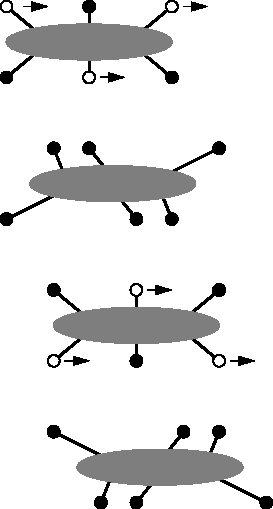
\includegraphics[width=0.2\columnwidth]{images/hexapod_static_walking_gait.pdf}
    \end{center}

    Un gait es una secuencia de eventos de elevación y liberación para las piernas individuales. Para un robot móvil con $k$ patas, el número total de secuencias de eventos distintas para una máquina para caminar es
    \begin{equation*}
        N = \left( 2k - 1\right)!
    \end{equation*}

    \note{Hay diferentes formas de desplazarse}
\end{frame}

\begin{frame}
    \frametitle{Tipos de Ruedas}

	\begin{figure}[!h]
        \centering
        \subfloat[Fija]
        {
            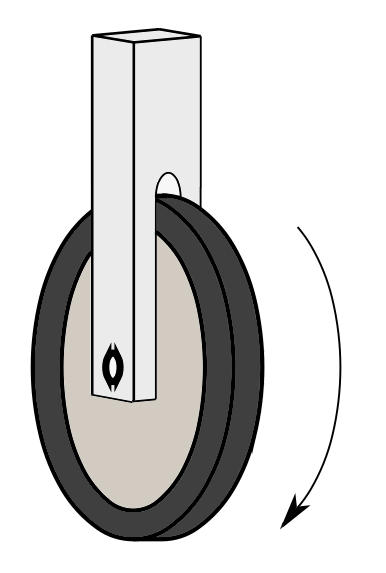
\includegraphics[width=0.15\columnwidth]{./images/fix_wheel.png}
        }
        \subfloat[Direccional]
        {
            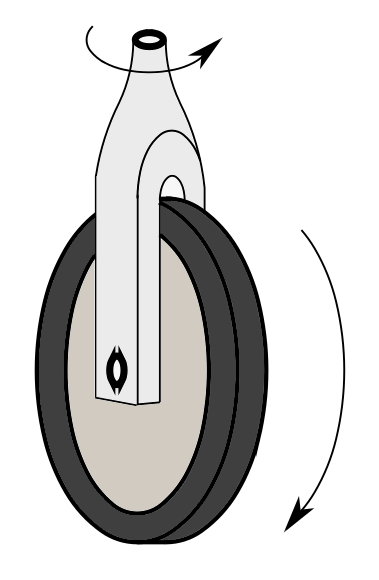
\includegraphics[width=0.15\columnwidth]{./images/directional_wheel.png}
        }
        \subfloat[Giratoria]
        {
            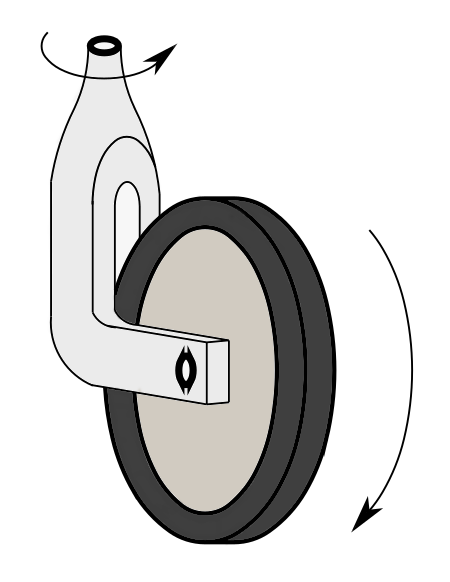
\includegraphics[width=0.15\columnwidth]{./images/rotational_wheel.png}
        }
        \subfloat[Omnidireccional]
        {
            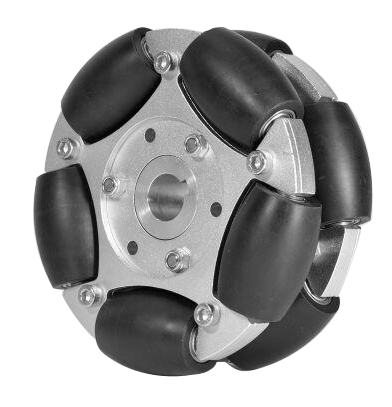
\includegraphics[width=0.2\columnwidth]{./images/omni_wheel.png}
        }
        \subfloat[Mecanum]
        {
            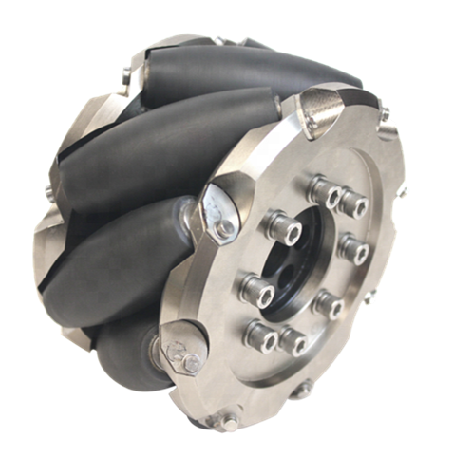
\includegraphics[width=0.2\columnwidth]{./images/mecanum_wheel.png}
        }
    \end{figure}
\end{frame}

\begin{frame}
    \frametitle{Configuraciones de robots con ruedas}

    \begin{figure}[!h]
        \centering
        \subfloat[Diff-drive]
        {
            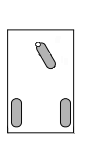
\includegraphics[height=0.3\textheight]{./images/differential_drive_robot.png}
        }
        \subfloat[Skid-steer]
        {
            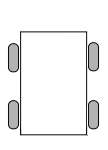
\includegraphics[height=0.3\textheight]{./images/skid_steer_robot.png}
        }
        \subfloat[Triciclo]
        {
            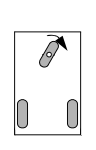
\includegraphics[height=0.3\textheight]{./images/tricycle_robot.png}
        }
        \subfloat[Car-like]
        {
            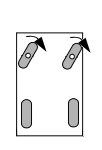
\includegraphics[height=0.3\textheight]{./images/carlike_robot.png}
        }\\
        \subfloat[Omni-wheel]
        {
            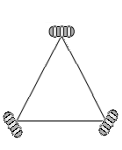
\includegraphics[height=0.3\textheight]{./images/omni_robot.png}
        }
        \subfloat[Mecanum]
        {
            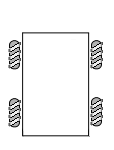
\includegraphics[height=0.3\textheight]{./images/mecanum_robot.png}
        }
    \end{figure}
\end{frame}


\begin{frame}
    \frametitle{Drones?}

\end{frame}